\subsection{Control problem}
\label{sec:controlproblem}

A sketch of the full system can be seen on figure \ref{fig:controlsch}.
The key to control the system resides in finding a good motor actuation in order to keep  the systems center of gravity close to the equilibrium as possible.
The center of gravity is marked by the dot at the end of the line of the segway in figure \ref{fig:controlsch}.
For convenience this is also in the sketch aligned with the IMUs axis.

In order to have a stable system, then the line from the center of gravity of the system to the wheels axis should be perpendicular to the ground plane.
There are different possibilities to control this system.
The chosen implementation uses as error signal the acceleration in the x-axis of the accelerometer, knowing that its value should be close to zero when at the stable position.

\begin{figure}[H]
\centering
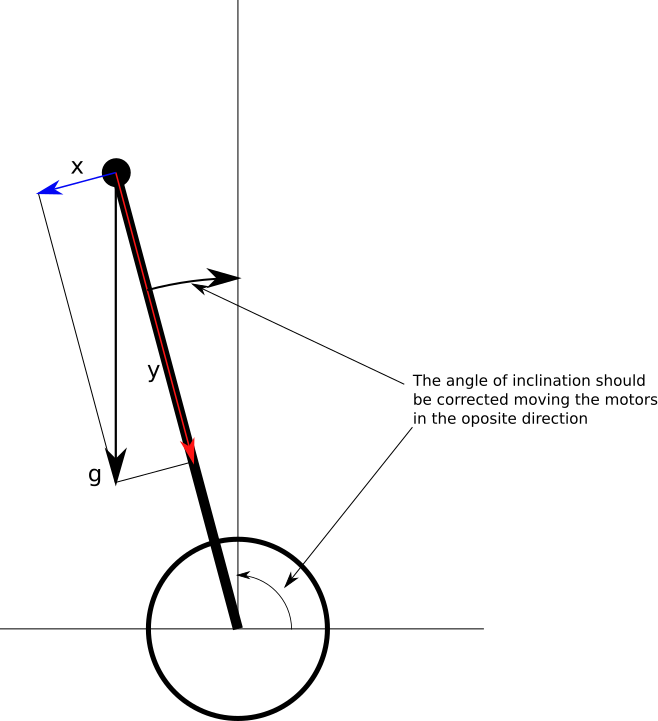
\includegraphics[width = 0.5 \textwidth]{images/segway_scheme}
\caption[Sketch of physical system.]{Sketch of the physical system. The values x and y are the readings on the accelerometer on the corresponding axis.}
\label{fig:controlsch}
\end{figure}

In this case, it is difficult to estimate the gravity center of the robot and then a optimal PID model.
It is, however, possible to obtain an acceptable control by tuning manually the PID.
%Using this approach it is however noticeable that the measured error along the x-axis will be higher than caused by the gravitational force when it is accelerating in the fall.

More advanced approaches try to estimate the angle of tilt.
These approaches require calculations including the use of trigonometric functions implemented on the FPGA.
This is why the simpler approach was used as the FPGA in use has a very limited block RAM so the functions can not be stored as a direct lookup, but should be calculated on runtime.